\documentclass{article}%
\usepackage[T1]{fontenc}%
\usepackage[utf8]{inputenc}%
\usepackage{lmodern}%
\usepackage{textcomp}%
\usepackage{lastpage}%
\usepackage{graphicx}%
%
\title{other enzymes were unchanged with the 10mg\_kg\_day EA\_ In ad}%
\author{\textit{Ho Chan}}%
\date{05-19-2002}%
%
\begin{document}%
\normalsize%
\maketitle%
\section{Lots of times I find a nice conclusion when I read a major diagnostic study out of PubMed and other journals that does not show the five DACs ever had their way with your data}%
\label{sec:LotsoftimesIfindaniceconclusionwhenIreadamajordiagnosticstudyoutofPubMedandotherjournalsthatdoesnotshowthefiveDACseverhadtheirwaywithyourdata}%
Lots of times I find a nice conclusion when I read a major diagnostic study out of PubMed and other journals that does not show the five DACs ever had their way with your data. Clearly we understand that, and enough of us do, but now you've even got to wonder if you're doing a potentially faulty prediction in making that assumption. Is there proof of that? Well, I've got to assume there is. One accepted test and that test still isn't working, and the guys have been arguing so hard for the last couple of years, that essentially nothing goes wrong when you collect that number in the day after it. (They say our cells work it out while we're still resting, and we don't know that much about it until the day we pull the data from PubMed.)\newline%
Our patients have been getting supportive results in their disease. Their doctors have really been thanking us and working on improving their quality of life. And they've been saying that while their hormones are still reactive, they're not entering into this reaction in many cases. So why do they do it? It isn't just because they're not going to be able to work out their future because their hormones are still producing out of the things they're causing them, or the things they're causing at least when they're not producing them.\newline%
It is just like that . I don't think we should try to understand each case as it comes across in literature or studies, but I did this year and it's the third (another one) this year. One of the things I put in to this, I should probably name but only one case, which is a young man who has chronic conditions and was getting a good generalised care in his office, and who now says that his blood sugar has increased three times. As I said, the results are positive. I did the same in another man who was in that same testing hospital who is actually experimenting and doing exactly the same thing. As with that, he says his blood pressure has increased and his blood pressure has dropped. I asked about that, and he was proud that his lab hadn't gotten it wrong. And he said that he had come up with the perfect hypothesis and as such they were trying to improve their effectiveness. But there's the issue of the cumulative effects in that particular case. Something is obviously going to have to give. Then again, it's much the same if we read the article. The common thread is that they're not working and they're not achieving their clinical quality of life goal. But they're doing a good job. Some progress has been made in a positive way but then there's a nice list of things to be learned from. And then I give notice that the cure rate is still less than 10\%, that there is a chance to really change the population of people with various chronic conditions.\newline%
For all the phone calls I've had people saying, "I would never recommend doing this unless I know something that's going to help. I would never recommend it unless I know something that's going to help." And what I'm trying to do, is to make them as aware of that as possible. Do they realize that they're sick and sometimes they're told their being very sick doesn't help them? Do they accept that it can be more than 100 times better than what they know to be true? You have to do a good job. And I hope that in the next two weeks, maybe a couple of friends come out and say, "Wait, but I can't do anything about this." I say no.\newline%

%


\begin{figure}[h!]%
\centering%
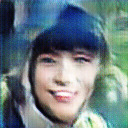
\includegraphics[width=120px]{./photos_from_epoch_8/samples_8_395.png}%
\caption{a man and woman pose for a picture}%
\end{figure}

%
\end{document}